\section{Reliability and availability}

Dependability can be subdivided into the following components:
\begin{figure}[H]
    \centering
    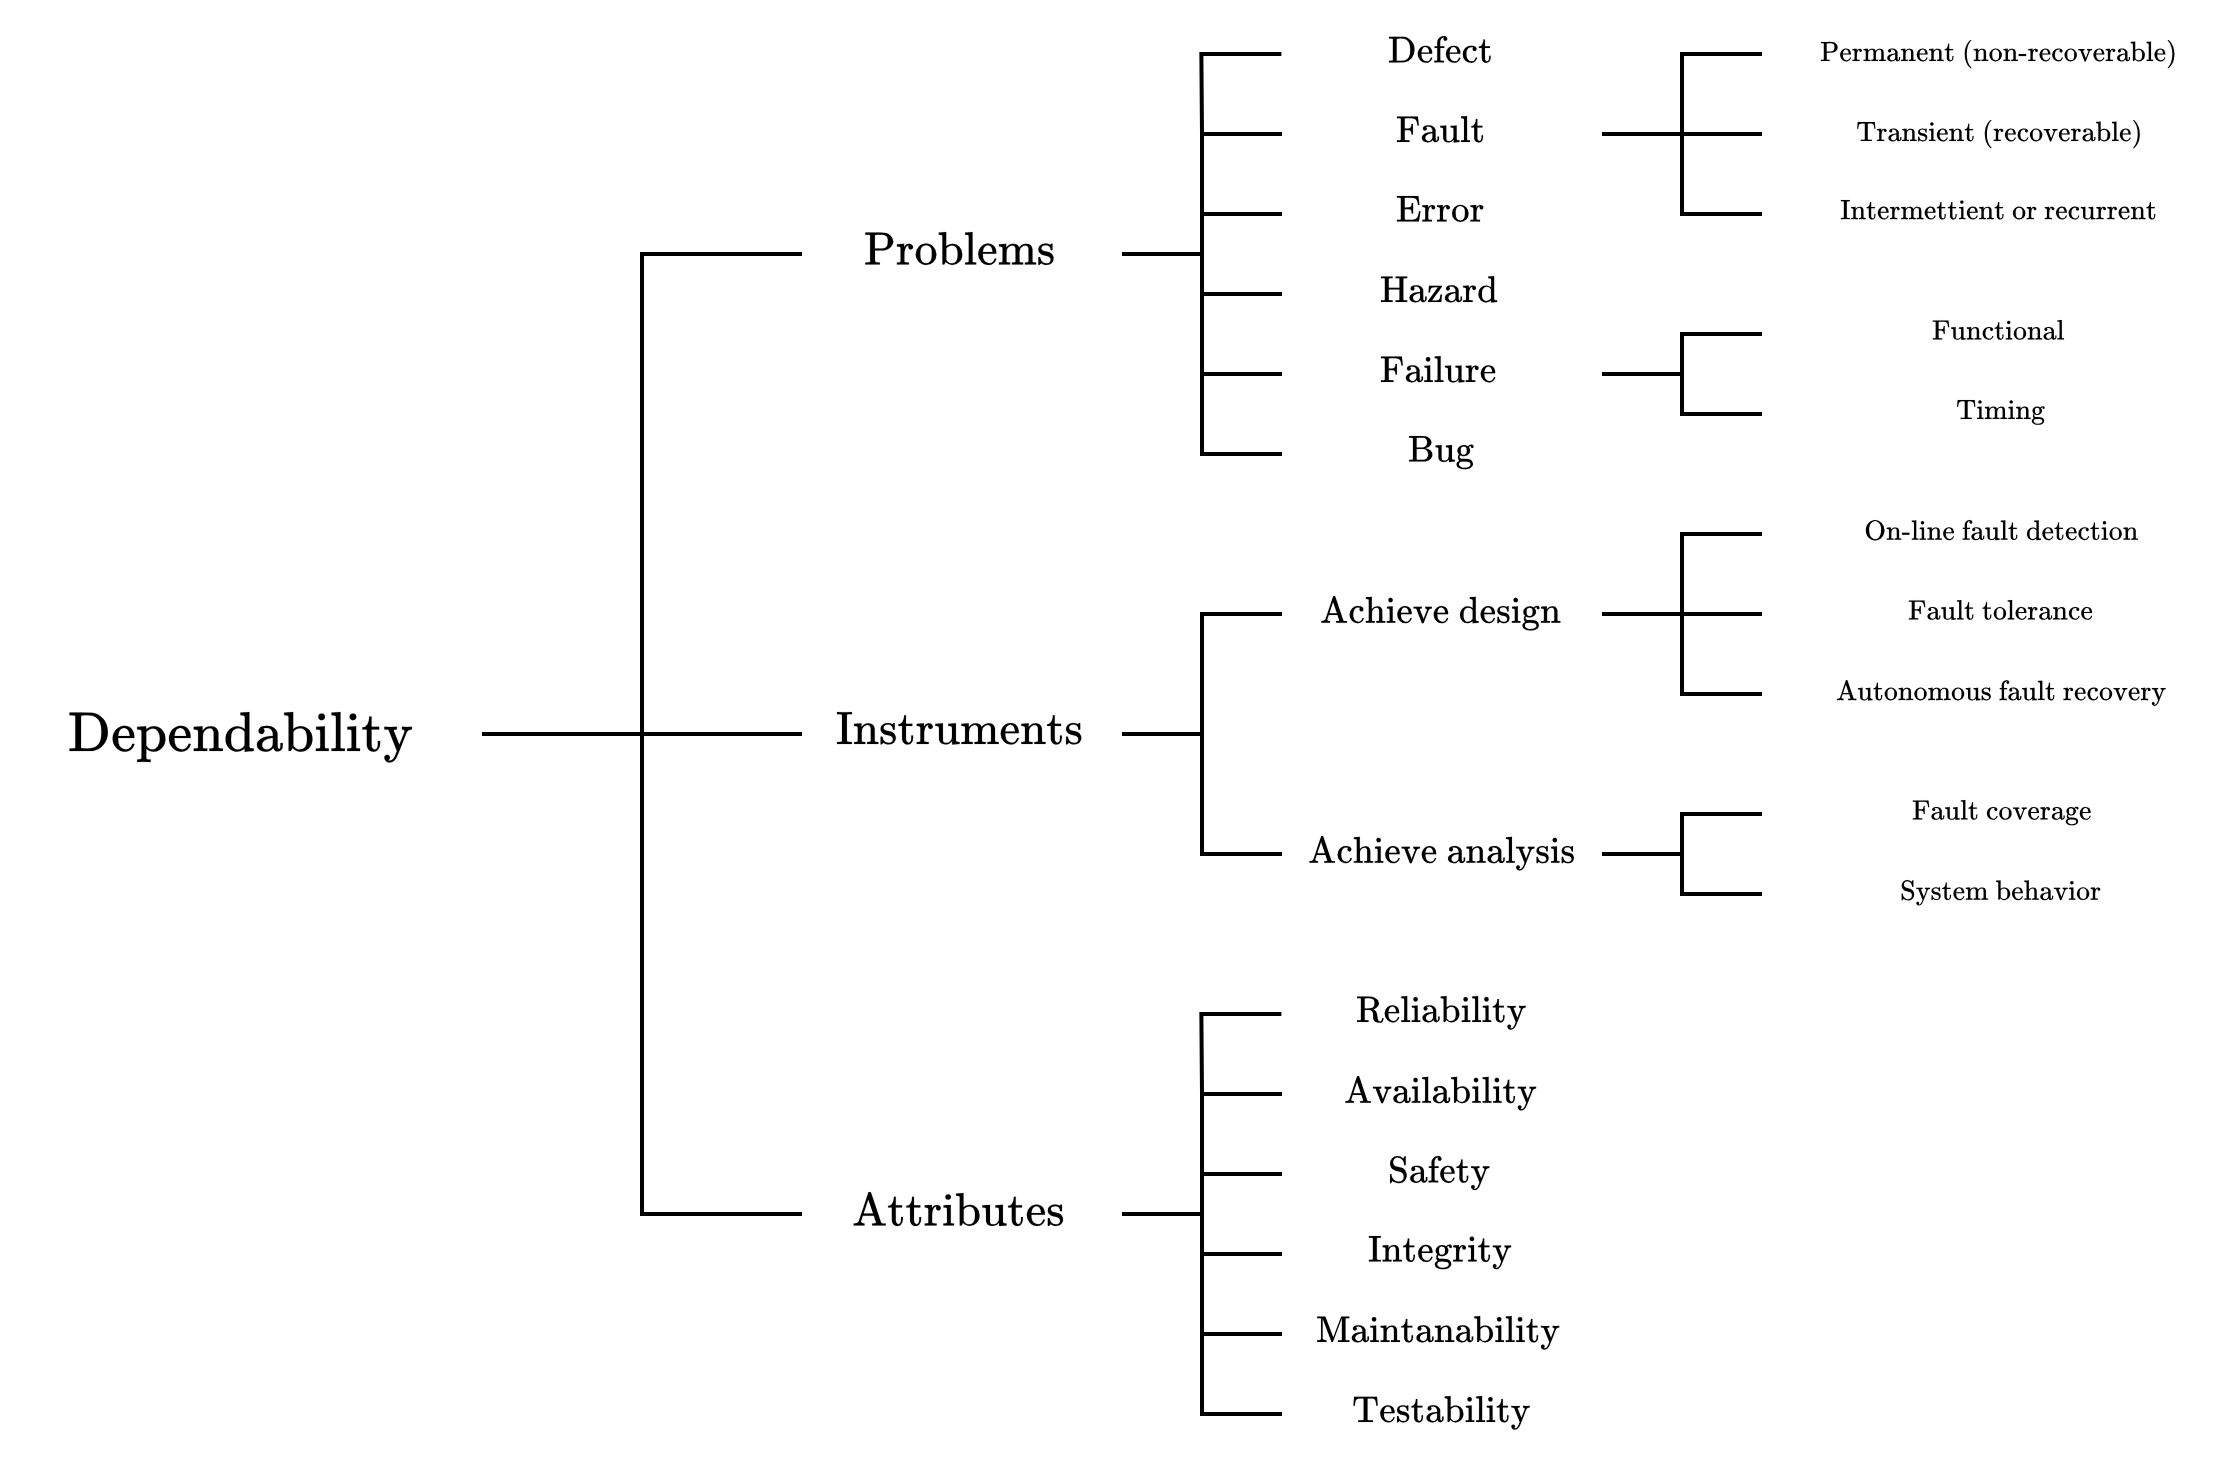
\includegraphics[width=0.6\linewidth]{images/dep1.png}
    \caption{Dependability components}
\end{figure}

\subsection{Reliability}
\begin{definition}[\textit{Reliability}]
    Reliability is the ability of a system or component to perform its required functions under stated conditions for a specified period of time.
\end{definition}
Reliability is denoted as the probability that the system operates correctly in a given environment until time $t$, expressed as:
\[R(t)=\Pr(\text{not failed during }[0,t])\]
Reliability is a monotonically decreasing function ranging from one to zero. 
This metric is often applied to systems where even brief periods of malfunction are intolerable or those that are difficult or impossible to repair.

Unreliability is the complementary measure to reliability, calculated as:
\[U_R(t)=1-R(t)\]

\subsection{Availability}
\begin{definition}[\textit{Availability}]
    Availability is the degree to which a system or component is operational and accessible when required for use.
\end{definition}
Availability is denoted as the probability that the system will be operational at time $t$: 
\[A(t)=\Pr(\text{not failed at time }t)=\dfrac{\text{Uptime}}{\text{Uptime}+\text{Downtime}}\]

Unavailability is the complementary measure to availability, calculated as:
\[U_A(t)=1-A(t)\]

\subsection{Other indices}
\begin{definition}[\textit{Repairable system}]
    A system is said to be repairable if $A(t) > R(t)$. 
\end{definition}
\begin{definition}[\textit{Unrepairable system}]
    A system is said to be unrepairable if $A(t) = R(t)$. 
\end{definition}
\begin{definition}[\textit{Mean Time To Failure}]
    The Mean Time To Failure (MTTF) represents the average duration before any failure occurs.
\end{definition}
MTTF can also be calculated as the integral of reliability:
\[\text{MTTF}=\int_0^\infty R(t)dt=\dfrac{\text{total operating time}}{\text{number of failures}}\]
\begin{definition}[\textit{Mean Time Between Failures}]
    The Mean Time Between Failures (MTBF) denotes the average duration between two consecutive failures.
\end{definition}
\begin{definition}[\textit{Failures In Time}]
    Failures In Time (FIT) refer to the reciprocal of the MTBF:
    \[\lambda=\dfrac{\text{number of failures}}{\text{total operating time}}\]
\end{definition}
\begin{figure}[H]
    \centering
    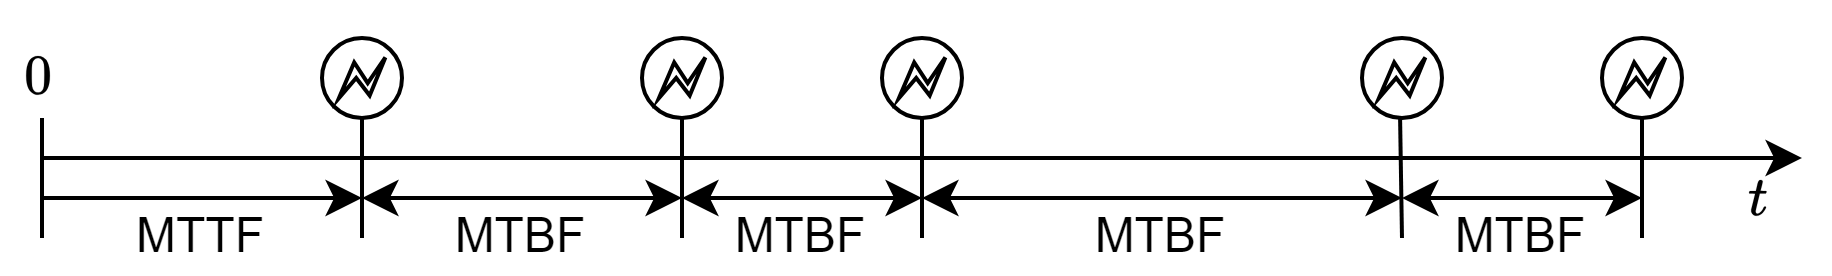
\includegraphics[width=0.75\linewidth]{images/mttb.png}
    \caption{MTTF and MTBF}
\end{figure}
\begin{definition}[\textit{Infant mortality}]
    Infant mortality measures failures occurring in new systems, often observed during testing phases.
\end{definition}
\begin{definition}[\textit{Random failures}]
    Random failures occur sporadically throughout the lifespan of a system.
\end{definition}
\begin{definition}[\textit{Wear out}]
    Wear out refers to the failure of components at the end of their operational life, potentially leading to system failure. 
\end{definition}
\begin{figure}[H]
    \centering
    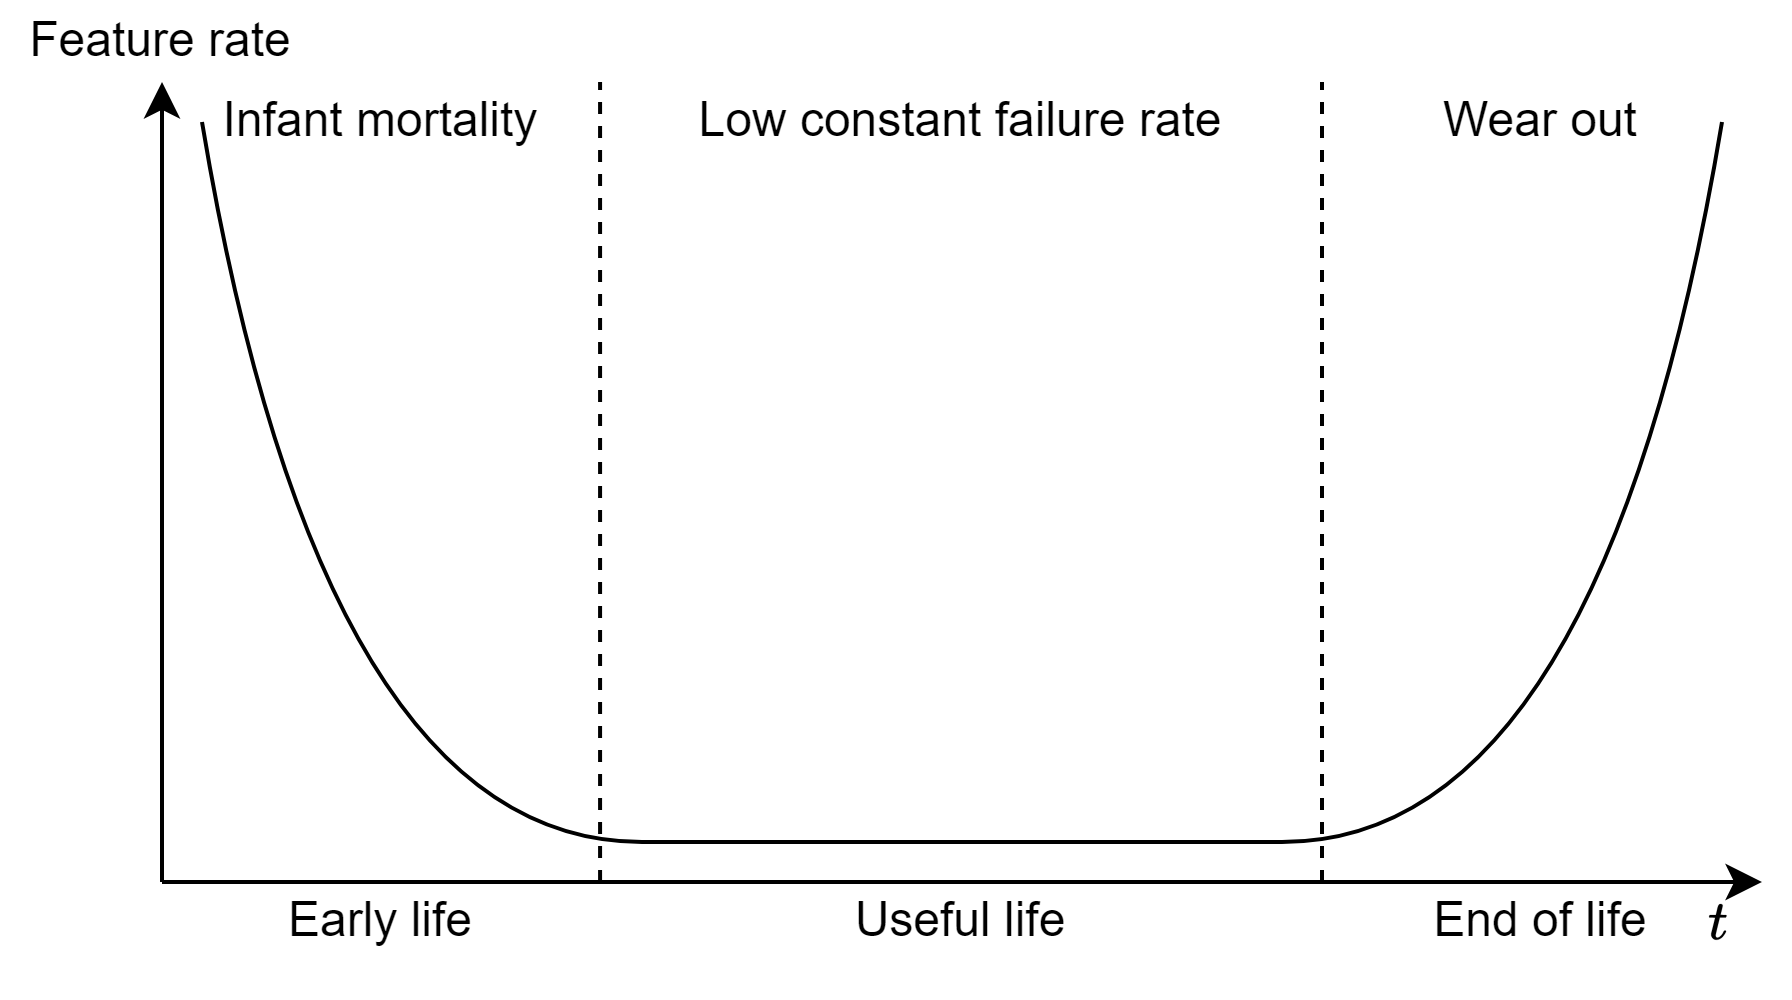
\includegraphics[width=0.55\linewidth]{images/dep2.png}
    \caption{Product reliability curve}
\end{figure}

\subsection{Defect identification}
To identify defective products and determine the MTTF, a burn-in test can be conducted. 
During this test, the system is subjected to elevated levels of temperature, voltage, current, and humidity to accelerate wear and tear.

In scenarios where systems exhibit low reliability but must remain operational, quick repairs of system failures that do not compromise data integrity may help mitigate the impact of low reliability. 
However, ensuring high reliability in systems can pose greater challenges.

Using information from the reliability function allows for the computation of a complex system's reliability over time, representing its expected lifetime.
\begin{definition}[\textit{Fault}]
    A fault is a defect within the system.
\end{definition}
\begin{definition}[\textit{Error}]
    An error is a deviation from the intended operation of the system or subsystem.
\end{definition}
\begin{definition}[\textit{Failure}]
    A failure occurs when the system is unable to perform its designated function.
\end{definition}
\begin{figure}[H]
    \centering
    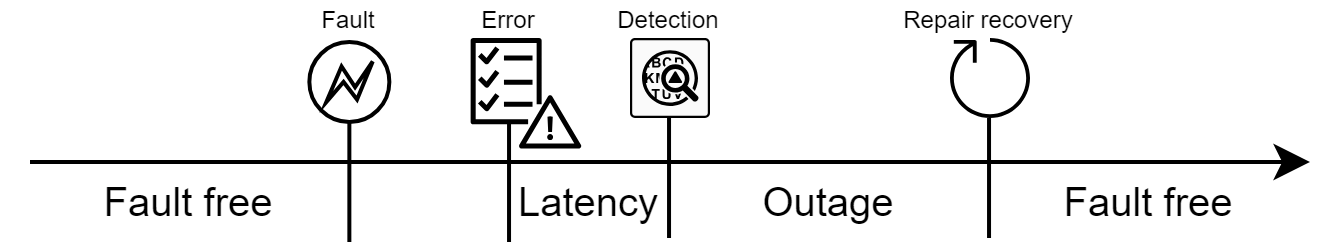
\includegraphics[width=0.75\linewidth]{images/rel.png}
    \caption{Reliability measures}
\end{figure}

\subsection{Block Diagrams}
Block diagrams provide an inductive model where a system is partitioned into blocks representing distinct elements such as components or subsystems. 
Each block has its own reliability or availability, which can be previously calculated or modeled. 
These blocks are then combined to represent all possible success paths within the system.

\paragraph*{Reliability Block Diagram}
The block reliability can be defined as:
\[R(t)=\Pr(T \geq t)=e^{-\lambda t}\]
Reliability Block Diagrams (RBD) provide an approach to compute the reliability of a system based on the reliability of its components.

In RBD, the elements can be connected in two ways:
\begin{itemize}
    \item \textit{Series}: all components must be operational for the system to function properly. 
        For systems with $n$ blocks in series, the total reliability is:
        \[R_S(t)=\prod_{i=1}^{n}R_i(t)=\prod_{i=1}^{n}e^{-\lambda_i t}\]
    \item \textit{Parallel}:  at least one component is operational, the system functions properly. 
        For systems with $n$ blocks in parallel, the total reliability is:
        \[R_S(t)=1-\prod_{i=1}^{n}\left(1-R_i(t)\right)=1-\prod_{i=1}^{n}\left(1-e^{-\lambda_i t}\right)\]
\end{itemize}

\paragraph*{Availability Block Diagram}
Availability Block Diagrams, the elements can be connected in two ways:
\begin{itemize}
    \item \textit{Series}: all components must be operational for the system to function properly. 
        For systems with $n$ blocks in series, the total availability is:
        \[A_S(t)=\prod_{i=1}^{n}A_i(t)=\prod_{i=1}^{n}\dfrac{\text{MTTF}_i}{\text{MTTF}_i+\text{MTTR}_i}\]
    \item \textit{Parallel}: if at least one component is operational, the system functions properly. 
        For systems with $n$ blocks in parallel, the total availability is:
        \[A_S(t)=1-\prod_{i=1}^{n}\left(1-A_i(t)\right)=1-\prod_{i=1}^{n}\left(1-\dfrac{\text{MTTF}_i}{\text{MTTF}_i+\text{MTTR}_i}\right)\]
\end{itemize}

\subsection{Redundancy}
A system may consist of two parallel replicas, where the primary replica operates continuously, and the redundant replica is activated only when the primary replica fails.

For operational redundancy, the system requires a mechanism to ascertain whether the primary replica is functioning correctly (online self-check) and a dynamic switching mechanism to deactivate the primary replica and activate the redundant one.
A system with one primary replica and $n$ redundant replicas (identical and perfectly switchable) can be represented by the reliability function:
\[R_S(t)=e^{-\lambda t}\sum_{i=0}^{n-1}\dfrac{{\left(\lambda t\right)}^i}{i!}\]

For a system comprising $n$ identical replicas where at least $r$ replicas must function correctly for the entire system to operate correctly, the reliability is computed as:
\[R_S(t)=R_V(t)\sum_{i=r}^{n}R(t)^i{(1-R(t))}^{n-i}\binom{n}{i}\]
Here, $R(t)$ denotes the component reliability, and $R_V(t)$ signifies the switching reliability.